\chapter{Permutazione, Ordinamento e Multiway Merge Sort in Memoria Esterna}
\label{cha:lecture-three}

\begin{center}
  \textbf{Lezione 3}\\
  \emph{Permutazione vs Ordinamento, Multiway Merge Sort, Snow Plow e Disk Striping}\\[0.5em]
  Data: 18 Settembre 2026
\end{center}

In questo capitolo viene esaminata la fondamentale relazione tra il problema della permutazione e quello dell'ordinamento nel modello di memoria a due livelli, confrontando i limiti del modello RAM con le gerarchie a blocchi. Viene introdotto e analizzato il Binary Merge Sort esterno evidenziandone i vincoli di sottoutilizzo, per poi sviluppare in dettaglio il \textit{Multiway Merge Sort} ($k$-Way Merge Sort) che raggiunge il lower bound asintotico di Aggarwal e Vitter. Vengono infine approfondite due tecniche cardine dell'Algorithm Engineering su memoria secondaria: l'ottimizzazione dei run iniziali mediante \textit{Snow Plow} (\textit{Replacement Selection}) e la scalabilità parallela su più dischi mediante \textit{Disk Striping}.


\section{Il Problema della Permutazione vs. Ordinamento}
\label{sec:permutation-vs-sorting}

\subsection{Formulazione del Problema}
\label{subsec:problem-formulation}

Siano dati due vettori di dimensione $n$:
\begin{itemize}
  \item Un array di dati $S[1 \dots n]$.
  \item Un vettore di permutazione $\pi[1 \dots n]$, contenente una permutazione biiettiva degli indici $\{1, 2, \dots, n\}$.
\end{itemize}

L'obiettivo consiste nel riordinare gli elementi di $S$ in un nuovo array $S'$ in modo tale che ogni elemento originario $S[i]$ sia ricollocato nella posizione target indicata da $\pi[i]$, ovvero:
\begin{equation}
  S'[\pi[i]] = S[i], \qquad \forall i \in \{1, \dots, n\}.
\end{equation}

\begin{example}[Permutazione di indici]
\label{ex:permutation-def}
Consideriamo un array di $4$ elementi e il relativo vettore di permutazione:
\begin{align*}
  \text{Indici:} \quad & 1 \quad 2 \quad 3 \quad 4 \\
  S = \quad & [\, A, \quad B, \quad C, \quad D \,] \\
  \pi = \quad & [\, 3, \quad 1, \quad 2, \quad 4 \,]
\end{align*}
Applicando la definizione elemento per elemento:
\begin{align*}
  S'[\pi[1]] &= S'[3] = A, \\
  S'[\pi[2]] &= S'[1] = B, \\
  S'[\pi[3]] &= S'[2] = C, \\
  S'[\pi[4]] &= S'[4] = D.
\end{align*}
L'array permutato finale risulta pertanto:
\[
  S' = [\, B, \quad C, \quad A, \quad D \,].
\]
\end{example}

In \autoref{fig:permutation-example} viene illustrata visivamente la mappatura degli elementi dall'array originale al vettore permutato.

\begin{figure}[htbp]
  \centering
  \begin{tikzpicture}[
    box/.style={draw, thick, minimum width=1.45cm, minimum height=0.72cm, align=center, font=\small},
    hdr/.style={font=\small\bfseries, anchor=east},
    arr/.style={-{Stealth[scale=1.1]}, thick}
  ]
    % Intestazioni riga a sinistra
    \node[hdr] at (-0.6, 2.8) {Indice $i$:};
    \node[hdr] at (-0.6, 2.0) {Elemento $S[i]$:};
    \node[hdr] at (-0.6, 1.2) {Target $\pi[i]$:};

    % Colonne dell'array originale S e vettore pi
    \foreach \x/\i/\val/\dest in {0.5/1/A/3, 2.7/2/B/1, 4.9/3/C/2, 7.1/4/D/4} {
      \node[box, fill=gray!8] (idx\i) at (\x, 2.8) {$i = \i$};
      \node[box, fill=blue!12] (S\i) at (\x, 2.0) {\textbf{\val}};
      \node[box, fill=orange!15] (P\i) at (\x, 1.2) {$\pi[\i] = \dest$};
    }

    % Intestazioni riga per array permutato S'
    \node[hdr] at (-0.6, -1.8) {Array $S'$:};
    \node[hdr] at (-0.6, -2.6) {Indice $j$:};

    % Celle dell'array permutato S'
    \foreach \x/\j/\val in {0.5/1/B, 2.7/2/C, 4.9/3/A, 7.1/4/D} {
      \node[box, fill=green!15] (Sp\j) at (\x, -1.8) {\textbf{\val}};
      \node[box, fill=gray!8] (tgt\j) at (\x, -2.6) {$j = \j$};
    }

    % Frecce di ricollocazione con etichette chiare su sfondo bianco
    \draw[arr, color=blue!75!black] (P1.south) to[out=270,in=90] 
      node[pos=0.45, right=1pt, font=\scriptsize, fill=white, inner sep=1.5pt] {$S[1] \to S'[3]$} (Sp3.north);

    \draw[arr, color=red!75!black] (P2.south) to[out=270,in=90] 
      node[pos=0.45, left=1pt, font=\scriptsize, fill=white, inner sep=1.5pt] {$S[2] \to S'[1]$} (Sp1.north);

    \draw[arr, color=orange!85!black] (P3.south) to[out=270,in=90] 
      node[pos=0.55, right=1pt, font=\scriptsize, fill=white, inner sep=1.5pt] {$S[3] \to S'[2]$} (Sp2.north);

    \draw[arr, color=teal!85!black] (P4.south) to[out=270,in=90] 
      node[pos=0.5, right=1pt, font=\scriptsize, fill=white, inner sep=1.5pt] {$S[4] \to S'[4]$} (Sp4.north);
  \end{tikzpicture}
  \caption{Mappatura della permutazione: ogni elemento $S[i]$ viene ricollocato nella posizione target specificata da $\pi[i]$ nell'array $S'$.}
  \label{fig:permutation-example}
\end{figure}

\subsection{Implementazione Ingenua su Modello RAM}
\label{subsec:naive-ram}

Nel modello RAM classico, in cui ogni accesso in lettura o scrittura a qualsiasi locazione di memoria ha costo unitario $\mathcal{O}(1)$, l'algoritmo si implementa tramite una singola scansione lineare:

\begin{algorithm}[H]
  \DontPrintSemicolon
  \KwInput{Array $S[1 \dots n]$, vettore di permutazione $\pi[1 \dots n]$}
  \KwOutput{Array $S$ permutato in loco}
  \For{$i \leftarrow 1$ \KwTo $n$}{
    $S'[\pi[i]] \leftarrow S[i]$\;
  }
  $S \leftarrow \mathrm{copy}(S')$\;
  \caption{Permutazione Diretta su RAM}
\end{algorithm}

La complessità temporale nel modello RAM è strettamente lineare:
\[
  T_{\mathrm{RAM}}(n) = \Theta(n).
\]
In memoria centrale, pertanto, permutare è asintoticamente più efficiente rispetto all'ordinamento basato su confronti, il quale richiede notoriamente un lower bound di $\Omega(n \log n)$ operazioni elementari.

\subsection{Principio di Simulazione (RAM contro Due Livelli)}
\label{subsec:simulation-principle}

\begin{theorem}[Teorema di Simulazione]
\label{thm:simulation}
Qualsiasi algoritmo sequenziale formulato per il modello RAM con complessità temporale $T(n)$ richiede al più $\mathcal{O}(T(n))$ trasferimenti di blocchi (I/O) nel modello di memoria a due livelli con parametri $(M, B)$.
\end{theorem}

\begin{proof}[Dimostrazione (Idea)]
Nel caso peggiore, ogni istruzione elementare RAM che effettua un accesso in memoria (lettura o scrittura) indirizza una locazione appartenente a un blocco non presente in memoria veloce $M$. Ciascun accesso scatena pertanto un trasferimento di blocco dal disco, producendo esattamente $1$ operazione di I/O. Moltiplicando il numero complessivo di passi $T(n)$ per il costo massimo di $1$ I/O per passo, si ottiene il bound superiore immediato di $\mathcal{O}(T(n))$ I/O.
\end{proof}

Sebbene il principio di simulazione garantisca che un algoritmo RAM possa sempre essere eseguito in memoria esterna, il bound $\mathcal{O}(T(n))$ è spesso inefficiente e lontano dall'ottimalità, poiché ignora completamente il fattore di aggregazione $B$ offerto dai trasferimenti a blocchi.

\subsection{La Relazione tra Ordinamento e Permutazione}
\label{subsec:relationship-sort-perm}

Nel modello a due livelli la gerarchia di complessità si ribalta, come sintetizzato nel prospetto comparativo in \autoref{tab:ram-vs-twlevel}:

\begin{table}[htbp]
  \centering
  \renewcommand{\arraystretch}{1.5}
  \begin{tabular}{lcc}
    \toprule
    \textbf{Problema} & \textbf{Modello RAM} & \textbf{Memoria a Due Livelli (I/O)} \\
    \midrule
    \textbf{Permutazione} $\operatorname{Perm}(n)$ & $\Theta(n)$ & $\Theta\big(\min\big\{ n, \, \operatorname{Sort}(n, M, B) \big\}\big)$ \\[0.4em]
    \textbf{Ordinamento} $\operatorname{Sort}(n)$ & $\Theta(n \log_2 n)$ & $\displaystyle \Theta\left(\frac{n}{B} \log_{M/B} \frac{n}{B}\right)$ \\
    \bottomrule
  \end{tabular}
  \caption{Confronto di complessità asintotica tra RAM e Memoria Esterna.}
  \label{tab:ram-vs-twlevel}
\end{table}

Per comprendere questa equivalenza nei sistemi a blocchi, consideriamo le due riduzioni:

\begin{enumerate}
  \item \textbf{Ordinamento tramite Permutazione:} Dato un array $S$, determinare la sequenza ordinata richiede dapprima di individuare la permutazione ordinante $\pi_S$ (calcolabile tramite ordinamento delle chiavi) e successivamente di applicare $\pi_S$ all'array $S$.
  \item \textbf{Permutazione tramite Ordinamento (Algoritmo a Riduzione di Coppie):}
  La permutazione di un array $S$ può essere trasformata in un problema di ordinamento di record secondo il seguente procedimento a tre stadi:
  \begin{itemize}
    \item \textbf{Passo 1 (Scansione e Creazione Coppie):} Si effettuano scansioni parallele e sequenziali di $S$ e $\pi$ per costruire una collezione di $n$ record composti dalla coppia $\langle S[i], \pi[i] \rangle$. Poiché si tratta di una scansione sequenziale lineare, il costo è:
    \[
      \mathrm{I/O}_{\text{Passo 1}} = \mathcal{O}\left(\frac{n}{B}\right).
    \]
    \item \textbf{Passo 2 (Ordinamento per Destinazione):} Si ordinano le $n$ coppie generate assumendo come chiave primaria la seconda componente $\pi[i]$. Il costo coincide esattamente con l'ordinamento in memoria esterna:
    \[
      \mathrm{I/O}_{\text{Passo 2}} = \operatorname{Sort}(n, M, B).
    \]
    \item \textbf{Passo 3 (Scansione ed Estrazione):} Avendo ordinato le coppie per indice di destinazione crescente, è sufficiente una scansione lineare per estrarre la prima componente $S[i]$, riversandola nel vettore finale $S'$. Costo:
    \[
      \mathrm{I/O}_{\text{Passo 3}} = \mathcal{O}\left(\frac{n}{B}\right).
    \]
  \end{itemize}
\end{enumerate}

Il costo I/O aggregato di questa strategia è:
\begin{equation}
  \mathrm{I/O}_{\text{Sort-based}} = \mathcal{O}\left(\frac{n}{B}\right) + \operatorname{Sort}(n, M, B) + \mathcal{O}\left(\frac{n}{B}\right) = \Theta(\operatorname{Sort}(n, M, B)).
\end{equation}

\begin{example}[Tracciamento della Riduzione a Coppie con Array Reali]
\label{ex:pair-reduction-trace}
Per visualizzare concretamente la riduzione, consideriamo i dati dell'\autoref{ex:permutation-def}:
\[
  S = [A, B, C, D], \qquad \pi = [3, 1, 2, 4].
\]
L'algoritmo opera attraverso tre stati successivi dell'array di record:
\begin{itemize}
  \item \textbf{Passo 1 (Accoppiamento):} Si accoppia sequenzialmente ciascun elemento con la propria coordinata target:
  \[
    P = \big[ \, \langle A, 3 \rangle, \;\; \langle B, 1 \rangle, \;\; \langle C, 2 \rangle, \;\; \langle D, 4 \rangle \, \big].
  \]
  \item \textbf{Passo 2 (Sort esterno su $\pi[i]$):} L'array viene ordinato assumendo come chiave di comparazione il secondo valore della tupla (la destinazione finale):
  \[
    P_{\text{ordinato}} = \big[ \, \langle B, \mathbf{1} \rangle, \;\; \langle C, \mathbf{2} \rangle, \;\; \langle A, \mathbf{3} \rangle, \;\; \langle D, \mathbf{4} \rangle \, \big].
  \]
  \item \textbf{Passo 3 (Estrazione sequenziale):} Proiettando la prima coordinata di ciascun elemento ordinato, si ricompone il vettore finale:
  \[
    S' = [B, C, A, D],
  \]
  che realizza esattamente la permutazione originaria poiché $S'[1]=B$, $S'[2]=C$, $S'[3]=A$, $S'[4]=D$.
\end{itemize}
\end{example}

La pipeline di riduzione delle coppie è illustrata graficamente in \autoref{fig:pair-reduction}.

\begin{figure}[htbp]
  \centering
  \begin{tikzpicture}[
    node distance=0.55cm and 0cm,
    data/.style={draw=blue!60!black, fill=blue!6, rounded corners=4pt, font=\small, align=center, inner sep=5pt, minimum width=6.2cm},
    stepnode/.style={draw=orange!80!black, fill=orange!10, rounded corners=4pt, font=\small\bfseries, align=center, inner sep=5pt, minimum width=7.2cm},
    outdata/.style={draw=teal!70!black, fill=teal!10, rounded corners=4pt, font=\small\bfseries, align=center, inner sep=5pt, minimum width=6.2cm},
    arr/.style={-{Stealth[scale=1.1]}, thick, draw=gray!70!black}
  ]
    \node[data] (in) {Dati di Input\\Array $S[1\dots n]$ \quad e \quad Vettore $\pi[1\dots n]$};
    \node[stepnode, below=of in] (s1) {Passo 1: Accoppiamento Sequenziale\\{\normalfont\footnotesize Costo: $\mathcal{O}(n/B)$ I/O (scansione lineare in streaming)}};
    \node[data, below=of s1] (pairs) {Collezione di Coppie Disordinate\\$\big\{ \langle S[i], \pi[i] \rangle \;\mid\; i = 1, \dots, n \big\}$};
    \node[stepnode, below=of pairs] (s2) {Passo 2: Ordinamento su Indice $\pi[i]$\\{\normalfont\footnotesize Costo: $\operatorname{Sort}(n, M, B)$ I/O (Merge Sort esterno)}};
    \node[data, below=of s2] (spairs) {Coppie Ordinate per Destinazione Crescente\\$\big\{ \langle S[\pi^{-1}[j]], j \rangle \;\mid\; j = 1, \dots, n \big\}$};
    \node[stepnode, below=of spairs] (s3) {Passo 3: Estrazione Sequenziale\\{\normalfont\footnotesize Costo: $\mathcal{O}(n/B)$ I/O (scrittura sequenziale)}};
    \node[outdata, below=of s3] (out) {Array Finale Permutato\\$S'[1\dots n]$ \quad con \quad $S'[\pi[i]] = S[i]$};

    \draw[arr] (in) -- (s1);
    \draw[arr] (s1) -- (pairs);
    \draw[arr] (pairs) -- (s2);
    \draw[arr] (s2) -- (spairs);
    \draw[arr] (spairs) -- (s3);
    \draw[arr] (s3) -- (out);
  \end{tikzpicture}
  \caption{Flusso operativo dell'algoritmo di permutazione basato sulla riduzione a coppie.}
  \label{fig:pair-reduction}
\end{figure}

\section{Complessità di Permutazione in Memoria Esterna}
\label{sec:permutation-complexity}

Il lower bound fondamentale per il problema della permutazione in memoria a due livelli è stato stabilito da Aggarwal e Vitter~\cite{aggarwal1988}:
\begin{equation}
  \operatorname{Perm}(n, M, B) = \Theta\left(\min\left\{ n, \, \frac{n}{B} \log_{M/B}\left(\frac{n}{B}\right) \right\}\right).
\end{equation}
Definendo $L = \log_{M/B}(n/B)$ come il numero di passate richieste dalla fusione multi-via nell'ordinamento:
\begin{equation}
  \operatorname{Sort}(n, M, B) = \Theta\left(\frac{n}{B} \cdot L\right).
\end{equation}

\subsection{Analisi dei Casi Limite}
\label{subsec:corner-cases}

Il confronto tra l'algoritmo ingenuo diretto e la strategia basata sull'ordinamento delle coppie dipende dal valore relativo tra la dimensione del blocco $B$ e il numero di livelli $L$:
\begin{itemize}
  \item \textbf{Caso 1 ($n \ge \frac{n}{B} \cdot L \iff B \ge L$):}  
  La dimensione del blocco $B$ è maggiore o uguale alla profondità dell'albero di fusione. In questa situazione, ordinare le coppie richiede meno I/O rispetto all'accesso casuale elemento per elemento:
  \[
    \operatorname{Perm}(n, M, B) = \Theta(\operatorname{Sort}(n, M, B)).
  \]
  \item \textbf{Caso 2 ($n < \frac{n}{B} \cdot L \iff B < L$):}  
  Se la dimensione del blocco fosse patologicamente piccola rispetto al volume complessivo dei dati ($B < L$), eseguire $n$ accessi diretti (al più $n$ I/O) risulterebbe asintoticamente inferiore al costo dell'ordinamento:
  \[
    \operatorname{Perm}(n, M, B) = \Theta(n).
  \]
\end{itemize}

\subsection{Verifica Numerica su Parametri Architetturali Reali}
\label{subsec:numerical-check}

Per comprendere quale dei due regimi asintotici si manifesti nei sistemi reali, consideriamo parametri architetturali realistici ed estremi:
\begin{itemize}
  \item Memoria interna veloce: $M = 16\text{ GB} = 2^4 \cdot 2^{30} \text{ elementi} = 2^{34}$ elementi.
  \item Dimensione del blocco disco: $B = 32\text{ KB} = 2^5 \cdot 2^{10} \text{ elementi} = 2^{15}$ elementi.
  \item Dimensione del dataset di input: $n = 2^{60}$ elementi (scala Exabyte).
\end{itemize}

Calcoliamo il numero di passate $L$:
\[
  L = \log_{M/B}\left(\frac{n}{M}\right) = \frac{\log_2(n / M)}{\log_2(M / B)}.
\]
Sostituendo i valori esponenziali:
\begin{align*}
  \frac{n}{M} &= \frac{2^{60}}{2^{34}} = 2^{26} \implies \log_2\left(\frac{n}{M}\right) = 26, \\
  \frac{M}{B} &= \frac{2^{34}}{2^{15}} = 2^{19} \implies \log_2\left(\frac{M}{B}\right) = 19.
\end{align*}
Otteniamo:
\[
  L = \frac{26}{19} \approx 1{,}36 < 2.
\]
Poiché $B = 2^{15} = 32\,768$ e $L \le 2$, la condizione $B \ge L$ è verificata con un margine di oltre quattro ordini di grandezza ($32\,768 \gg 2$). Di conseguenza, in qualsiasi sistema reale la permutazione è strettamente governata dal costo di ordinamento:
\[
  \operatorname{Perm}(n) = \Theta(\operatorname{Sort}(n)).
\]

\section{Binary Merge Sort in Memoria Esterna}
\label{sec:binary-merge-sort}

L'algoritmo ricorsivo classico di Merge Sort si estende alla memoria esterna suddividendo l'array in due metà, ordinando ricorsivamente ciascuna metà e fondendo i due sottoarray ordinati (\textit{runs}):

\begin{algorithm}[H]
  \DontPrintSemicolon
  \KwInput{Array $S$, estremi $i, j$}
  \KwOutput{Sottoarray $S[i \dots j]$ ordinato}
  \If{$i < j$}{
    $m \leftarrow \lfloor (i + j) / 2 \rfloor$\;
    $\mathrm{MS}(S, i, m)$\;
    $\mathrm{MS}(S, m + 1, j)$\;
    $\mathrm{MERGE}(S, i, m, j)$\;
  }
  \caption{Binary Merge Sort}
\end{algorithm}

\subsection{Architettura dei Buffer nella Procedura di Fusione}
\label{subsec:merge-procedure}

Dati due segmenti ordinati (\textit{runs}) consecutivi di lunghezza $l$, la procedura di fusione genera un unico run ordinato di lunghezza $2l$ su un array temporaneo $S'$.

\begin{itemize}
  \item \textbf{Nel Modello RAM:} Si effettuano al più $2l$ confronti e $2l$ trasferimenti in memoria, determinando un costo computazionale di $\Theta(l)$.
  \item \textbf{Nel Modello a Due Livelli:} Per eseguire la fusione minimizzando gli I/O, la memoria interna $M$ viene partizionata in $3$ buffer dedicati, ciascuno di dimensione esattamente pari a un blocco $B$:
  \begin{enumerate}
    \item \textbf{Input Buffer 1:} ospita un blocco (dimensione $B$) del primo run ordinato.
    \item \textbf{Input Buffer 2:} ospita un blocco (dimensione $B$) del secondo run ordinato.
    \item \textbf{Output Buffer:} raccoglie gli elementi fusi in ordine crescente fino al riempimento di un blocco $B$.
  \end{enumerate}
\end{itemize}

In \autoref{fig:merge-buffers} è rappresentata la gestione della memoria interna e dei flussi da/verso il disco durante la fusione binaria.

\begin{figure}[htbp]
  \centering
  \begin{tikzpicture}[
    buf/.style={draw, thick, fill=blue!10, minimum width=3.0cm, minimum height=1.1cm, align=center, font=\small},
    disk/.style={draw, thick, fill=gray!15, minimum width=3.0cm, minimum height=0.9cm, align=center, font=\small},
    arr/.style={-{Stealth[scale=1.1]}, thick}
  ]
    % Memoria Interna Container
    \draw[dashed, thick, color=blue!70!black, fill=blue!2] (-0.5, 1.8) rectangle (10.5, 3.8);
    \node[anchor=west, font=\bfseries\small, color=blue!70!black] at (-0.3, 3.5) {Memoria Interna $M$ (Spazio utilizzato: $3B$)};

    % Buffer interni
    \node[buf] (b1) at (1.5, 2.6) {Input Buffer 1\\(dimensione $B$)};
    \node[buf] (b2) at (5.0, 2.6) {Input Buffer 2\\(dimensione $B$)};
    \node[buf, fill=green!15] (bout) at (8.5, 2.6) {Output Buffer\\(dimensione $B$)};

    % Dischi / Run esterni
    \node[disk] (d1) at (1.5, 0.2) {Run 1 su Disco\\(lunghezza $l$)};
    \node[disk] (d2) at (5.0, 0.2) {Run 2 su Disco\\(lunghezza $l$)};
    \node[disk, fill=green!8] (dout) at (8.5, 0.2) {Run Fuso su Disco\\(lunghezza $2l$)};

    % Connessioni
    \draw[arr, color=blue!80!black] (d1) -- node[right, font=\scriptsize]{Read $B$} (b1);
    \draw[arr, color=blue!80!black] (d2) -- node[right, font=\scriptsize]{Read $B$} (b2);
    \draw[arr, color=green!60!black] (bout) -- node[right, font=\scriptsize]{Flush $B$} (dout);

    % Logica interna
    \draw[thick, dotted, color=gray!80!black] (b1.east) -- (b2.west);
    \draw[thick, dotted, color=gray!80!black] (b2.east) -- (bout.west);
  \end{tikzpicture}
  \caption{Architettura dei buffer di memoria interna durante la procedura di fusione binaria.}
  \label{fig:merge-buffers}
\end{figure}

Il funzionamento del protocollo di trasferimento è il seguente:
\begin{enumerate}
  \item Gli elementi in testa ai due buffer di input vengono confrontati in CPU; l'elemento minore viene spostato nell'output buffer.
  \item Quando uno dei buffer di input si svuota, viene emessa una lettura da disco per caricare il blocco successivo del rispettivo run ($\frac{l}{B}$ I/O per ciascun run di input).
  \item Non appena l'output buffer si riempie con $B$ elementi, viene scaricato (\textit{flushed}) su disco con una singola scrittura ($\frac{2l}{B}$ I/O complessivi di scrittura).
\end{enumerate}

Il costo aggregato della fusione di due run di lunghezza $l$ è:
\begin{equation}
  \mathrm{I/O}_{\text{Merge}}(l) = \frac{l}{B} + \frac{l}{B} + \frac{2l}{B} = \frac{4l}{B} = \Theta\left(\frac{l}{B}\right).
\end{equation}

\subsection{Complessità dell'Albero di Ricorsione}
\label{subsec:recursion-tree}

La ricorsione si arresta non appena la dimensione del sottoarray scende al di sotto della capacità della memoria interna $M$. A questo livello base, ciascun sottoarray di dimensione $M$ viene letto interamente in memoria, ordinato localmente tramite un algoritmo interno efficiente (es. QuickSort o HeapSort) con zero I/O aggiuntivi, e riscritto su disco con $\mathcal{O}(M/B)$ I/O.

Si generano così inizialmente:
\[
  N_{\mathrm{run}} = \frac{n}{M} \text{ run ordinati di dimensione } M.
\]
L'albero di fusione binaria presenta un'altezza complessiva pari a:
\begin{equation}
  h = \log_2\left(\frac{n}{M}\right) \text{ livelli}.
\end{equation}

In \autoref{fig:binary-merge-tree} è illustrata la struttura dell'albero di fusione per il Binary Merge Sort esterno.

\begin{figure}[htbp]
  \centering
  \resizebox{0.95\linewidth}{!}{%
  \begin{tikzpicture}[
    level 1/.style={sibling distance=3.6cm, level distance=1.2cm},
    level 2/.style={sibling distance=1.8cm, level distance=1.2cm},
    node/.style={draw=blue!70!black, rounded corners=3pt, fill=blue!8, font=\small, minimum width=1.5cm, minimum height=0.6cm, align=center},
    leaf/.style={draw=yellow!70!black, rounded corners=3pt, fill=yellow!25, font=\small, minimum width=1.4cm, minimum height=0.6cm, align=center},
    cost/.style={font=\small, text=blue!80!black, anchor=west},
    lbl/.style={font=\small\bfseries, text=gray!75!black, anchor=east}
  ]
    % Albero (centrato a x = -1.2)
    \node[node] at (-1.2, 0) (root) {Output: $n$}
      child { node[node] (n1) {Run $n/2$}
        child { node[leaf] (l1) {Run $M$} }
        child { node[leaf] (l2) {Run $M$} }
      }
      child { node[node] (n2) {Run $n/2$}
        child { node[leaf] (l3) {Run $M$} }
        child { node[leaf] (l4) {Run $M$} }
      };

    % Etichette di sinistra (anchor=east a x = -4.9: nessun contatto con l'albero)
    \node[lbl] at (-4.9, 0) {Livello $h$:};
    \node[lbl] at (-4.9, -1.2) {Livello 1:};
    \node[lbl] at (-4.9, -2.4) {Base ($n/M$ run):};

    % Linee tratteggiate verso i costi I/O
    \draw[dotted, thick, gray!50] (root.east) -- (2.3, 0);
    \node[cost] at (2.4, 0) {$\Theta(n/B)$ I/O};

    \draw[dotted, thick, gray!50] (n2.east) -- (2.3, -1.2);
    \node[cost] at (2.4, -1.2) {$\Theta(n/B)$ I/O};

    \draw[dotted, thick, gray!50] (l4.east) -- (2.3, -2.4);
    \node[cost] at (2.4, -2.4) {$\Theta(n/B)$ I/O};

    % Quota altezza albero con freccia rossa a x = 4.8
    \draw[thick, Stealth-Stealth, color=red!70!black] (4.8, 0.2) -- 
      node[right=3pt, font=\small, text=red!80!black, align=left]{$h = \log_2\left(\frac{n}{M}\right)$\\[2pt]livelli} 
      (4.8, -2.6);
  \end{tikzpicture}%
  }
  \caption{Albero di ricorsione del Binary Merge Sort esterno con indicazione dei costi I/O per livello.}
  \label{fig:binary-merge-tree}
\end{figure}

Ad ogni livello dell'albero di fusione, tutti gli $n$ elementi dell'array vengono scanditi esattamente una volta, richiedendo $\Theta(n/B)$ operazioni di I/O per livello. Moltiplicando per l'altezza dell'albero si ottiene la complessità totale:
\begin{equation}
  \mathrm{I/O}_{\text{BinaryMergeSort}} = \mathcal{O}\left(\frac{n}{B} \log_2\left(\frac{n}{M}\right)\right).
\end{equation}

\subsection{Criticità e Limiti di Efficienza}
\label{subsec:suboptimality}

Nonostante l'algoritmo migliori drasticamente rispetto a un approccio ingenuo, esso presenta un grave collo di bottiglia strutturale:
\begin{itemize}
  \item \textbf{Sottoutilizzo drastico della memoria interna:} Durante la fusione binaria vengono occupati contemporaneamente soltanto $3$ blocchi ($3B$ elementi) all'interno dello spazio disponibile $M$. Tutta la restante porzione di memoria interna $(M - 3B)$ rimane completamente inutilizzata.
  \item \textbf{Base del logaritmo sub-ottimale:} La base del logaritmo è rigidamente ancorata a $2$, mentre la memoria $M$ permetterebbe di mantenere aperti simultaneamente fino a:
  \[
    k \approx \frac{M}{B} - 1 \text{ buffer di input}.
  \]
  \item \textbf{Perdita del fattore di convergenza $\log_2(M/B)$:} La mancata estensione a una fusione a $k$ vie (\textit{Multiway Merge Sort}) comporta un numero di passate significativamente superiore, impedendo di raggiungere il lower bound ottimale:
  \[
    \mathcal{O}\left(\frac{n}{B} \log_{M/B}\left(\frac{n}{B}\right)\right).
  \]
\end{itemize}

In \autoref{fig:memory-utilization-comparison} viene evidenziata graficamente la disparità tra l'allocazione binaria e la piena saturazione della memoria veloce.

\begin{figure}[htbp]
  \centering
  \resizebox{0.95\linewidth}{!}{%
  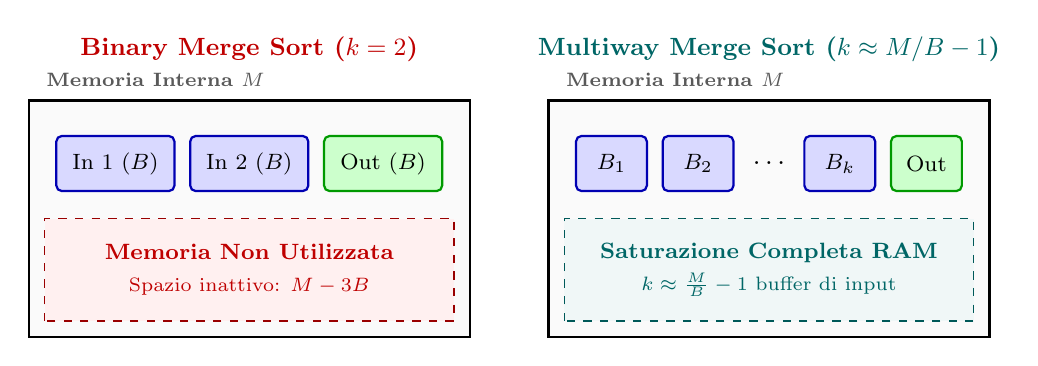
\begin{tikzpicture}[
    box/.style={draw, thick, rounded corners=2pt, align=center, font=\footnotesize},
    title/.style={font=\bfseries\small, align=center}
  ]
    % --- SINISTRA: Binary Merge Sort ---
    \node[title, color=red!75!black] at (2.8, 3.65) {Binary Merge Sort ($k=2$)};
    % Contenitore memoria interna M
    \draw[thick, fill=gray!4] (0, 0) rectangle (5.6, 3.0);
    \node[anchor=south west, font=\scriptsize\bfseries, color=gray!70!black] at (0.1, 3.05) {Memoria Interna $M$};

    % Buffer 1, 2, Out
    \node[box, fill=blue!15, draw=blue!70!black, minimum width=1.5cm, minimum height=0.7cm] at (1.1, 2.2) {In 1 ($B$)};
    \node[box, fill=blue!15, draw=blue!70!black, minimum width=1.5cm, minimum height=0.7cm] at (2.8, 2.2) {In 2 ($B$)};
    \node[box, fill=green!20, draw=green!60!black, minimum width=1.5cm, minimum height=0.7cm] at (4.5, 2.2) {Out ($B$)};

    % Area sprecata
    \draw[dashed, red!60!black, fill=red!6] (0.2, 0.2) rectangle (5.4, 1.5);
    \node[font=\footnotesize\bfseries, color=red!75!black, align=center] at (2.8, 0.85) {Memoria Non Utilizzata\\[2pt]{\normalfont\scriptsize Spazio inattivo: $M - 3B$}};

    % --- DESTRA: Multiway Merge Sort ---
    \node[title, color=teal!80!black] at (9.4, 3.65) {Multiway Merge Sort ($k \approx M/B - 1$)};
    % Contenitore memoria interna M
    \draw[thick, fill=gray!4] (6.6, 0) rectangle (12.2, 3.0);
    \node[anchor=south west, font=\scriptsize\bfseries, color=gray!70!black] at (6.7, 3.05) {Memoria Interna $M$};

    % Buffer multipli
    \node[box, fill=blue!15, draw=blue!70!black, minimum width=0.9cm, minimum height=0.7cm] at (7.4, 2.2) {$B_1$};
    \node[box, fill=blue!15, draw=blue!70!black, minimum width=0.9cm, minimum height=0.7cm] at (8.5, 2.2) {$B_2$};
    \node[font=\bfseries] at (9.4, 2.2) {$\dots$};
    \node[box, fill=blue!15, draw=blue!70!black, minimum width=0.9cm, minimum height=0.7cm] at (10.3, 2.2) {$B_k$};
    \node[box, fill=green!20, draw=green!60!black, minimum width=0.9cm, minimum height=0.7cm] at (11.4, 2.2) {Out};

    % Saturazione completa
    \draw[dashed, teal!70!black, fill=teal!6] (6.8, 0.2) rectangle (12.0, 1.5);
    \node[font=\footnotesize\bfseries, color=teal!80!black, align=center] at (9.4, 0.85) {Saturazione Completa RAM\\[2pt]{\normalfont\scriptsize $k \approx \frac{M}{B}-1$ buffer di input}};
  \end{tikzpicture}%
  }
  \caption{Confronto dell'efficienza nell'allocazione della memoria interna: grave sottoutilizzo nel Binary Merge Sort rispetto alla saturazione ottimale nel Multiway Merge Sort.}
  \label{fig:memory-utilization-comparison}
\end{figure}

Il superamento di questa limitazione strutturale conduce in modo naturale all'architettura dell'ordinamento multi-via, analizzata in dettaglio nelle sezioni seguenti.

\section{Equivalenza Asintotica del Costo di Ordinamento Esterno}
\label{sec:sorting-cost-equivalence}

Nella trattazione della complessità computazionale in memoria secondaria, il costo I/O dell'ordinamento esterno viene espresso nella letteratura specializzata~\cite{aggarwal1988} attraverso due notazioni apparentemente distinte:
\begin{equation}
  \Theta\left(\frac{n}{B} \log_{M/B}\left(\frac{n}{M}\right)\right)
  \qquad \text{oppure} \qquad
  \mathcal{O}\left(\frac{n}{B} \log_{M/B}\left(\frac{n}{B}\right)\right).
\end{equation}
Queste due formulazioni sono asintoticamente perfettamente equivalenti per qualsiasi istanza $n \ge M$.

Per dimostrare formalmente l'equivalenza, applichiamo le proprietà fondamentali dei logaritmi espandendo l'argomento del termine $\log_{M/B}(n/B)$:
\begin{align}
  \log_{M/B}\left(\frac{n}{B}\right)
  &= \log_{M/B}\left(\frac{n}{M} \cdot \frac{M}{B}\right) \nonumber \\
  &= \log_{M/B}\left(\frac{n}{M}\right) + \log_{M/B}\left(\frac{M}{B}\right) \nonumber \\
  &= \log_{M/B}\left(\frac{n}{M}\right) + 1.
  \label{eq:log-equivalence}
\end{align}
Moltiplicando l'identità per il fattore comune $\frac{n}{B}$, otteniamo:
\begin{equation}
  \frac{n}{B} \log_{M/B}\left(\frac{n}{B}\right)
  = \frac{n}{B} \log_{M/B}\left(\frac{n}{M}\right) + \frac{n}{B}.
\end{equation}
Dal punto di vista algoritmico, il termine additivo lineare $\frac{n}{B}$ corrisponde esattamente alla passata iniziale (\textit{Passo 0}) necessaria alla formazione dei \textit{run} ordinati di partenza tramite caricamento e ordinamento in RAM. 

Allorché $n \gg M$, si ha $\log_{M/B}(n/M) \ge 1$, per cui il termine additivo $+1$ viene pienamente assorbito dalla costante nascosta nella notazione asintotica $\Theta$:
\begin{equation}
  \Theta\left(\frac{n}{B} \log_{M/B}\left(\frac{n}{B}\right)\right)
  = \Theta\left(\frac{n}{B} \left(\log_{M/B}\left(\frac{n}{M}\right) + 1\right)\right)
  = \Theta\left(\frac{n}{B} \log_{M/B}\left(\frac{n}{M}\right)\right).
\end{equation}
Ne consegue che è possibile utilizzare indifferentemente $\frac{n}{M}$ oppure $\frac{n}{B}$ all'interno dell'argomento logaritmico senza alterare la rigorosità dell'analisi.

\section{Multiway Merge Sort (\texorpdfstring{$k$}{k}-Way Merge Sort)}
\label{sec:multiway-merge-sort}

Nel \textit{Binary Merge Sort}, descritto nella \autoref{sec:binary-merge-sort}, si allocano simultaneamente soltanto 3 blocchi di memoria interna, lasciando inutilizzato lo spazio residuo $M - 3B$. Il \textbf{Multiway Merge Sort} (o ordinamento per fusione a $k$ vie) supera radicalmente questa inefficienza sfruttando l'intera capacità $M$ per fondere simultaneamente $k$ sequenze ordinate in un'unica passata (\textit{fan-in} pari a $k$).

\subsection{Configurazione e Architettura della Memoria Interna}
\label{subsec:multiway-memory-layout}

La memoria primaria $M$ viene partizionata in unità di trasferimento di dimensione $B$:
\begin{itemize}
  \item $k = \frac{M}{B} - 1$ \textbf{buffer di input}, ciascuno di capacità esattamente pari a un blocco $B$, associati stabilmente a ciascuno dei $k$ run attivi su memoria secondaria.
  \item $1$ \textbf{buffer di output}, anch'esso di capacità $B$, deputato ad accumulare progressivamente gli elementi risultanti in ordine crescente prima del trasferimento fisico su disco.
  \item Una struttura dati ausiliaria residente interamente in memoria interna: un \textbf{Min-Heap} (o coda di priorità) contenente $k$ nodi. Ciascun nodo memorizza la chiave corrente minima di uno dei $k$ blocchi attivi insieme all'identificatore del buffer di provenienza.
\end{itemize}

In \autoref{fig:multiway-merge-architecture} viene illustrato lo schema architettonico dei buffer e il flusso dei dati coordinato dal Min-Heap.

\begin{figure}[htbp]
  \centering
  \resizebox{0.95\linewidth}{!}{%
  \begin{tikzpicture}[
    buf/.style={draw=blue!70!black, thick, fill=blue!10, rounded corners=2pt, minimum width=2.4cm, minimum height=0.75cm, align=center, font=\small},
    heap/.style={draw=orange!80!black, thick, fill=orange!15, rounded corners=4pt, minimum width=2.8cm, minimum height=1.4cm, align=center, font=\small\bfseries},
    outbuf/.style={draw=green!60!black, thick, fill=green!15, rounded corners=2pt, minimum width=2.8cm, minimum height=0.75cm, align=center, font=\small\bfseries},
    disk/.style={draw=gray!70!black, thick, fill=gray!12, rounded corners=2pt, minimum width=3.2cm, minimum height=0.8cm, align=center, font=\small},
    arr/.style={-{Stealth[scale=1.1]}, thick}
  ]
    % Contenitore Memoria Interna
    \draw[thick, dashed, fill=blue!2, draw=blue!60!black] (-0.3, -0.2) rectangle (12.2, 5.0);
    \node[anchor=south west, font=\small\bfseries, color=blue!70!black] at (-0.2, 5.05) {Memoria Interna $M$ (Capacit\`a: $k+1$ blocchi)};

    % Buffer di input
    \node[buf] (b1) at (1.6, 4.1) {Buffer In $1$ ($B$)};
    \node[buf] (b2) at (1.6, 3.1) {Buffer In $2$ ($B$)};
    \node[font=\bfseries] at (1.6, 2.2) {$\vdots$};
    \node[buf] (bk) at (1.6, 1.2) {Buffer In $k$ ($B$)};

    % Dischi di input
    \node[disk] (d1) at (-4.2, 4.1) {Run Attivo $1$ (Disco)};
    \node[disk] (d2) at (-4.2, 3.1) {Run Attivo $2$ (Disco)};
    \node[disk] (dk) at (-4.2, 1.2) {Run Attivo $k$ (Disco)};

    \draw[arr, color=blue!80!black] (d1) -- node[above, font=\scriptsize]{Read $B$} (b1);
    \draw[arr, color=blue!80!black] (d2) -- node[above, font=\scriptsize]{Read $B$} (b2);
    \draw[arr, color=blue!80!black] (dk) -- node[above, font=\scriptsize]{Read $B$} (bk);

    % Min-Heap al centro
    \node[heap] (hp) at (6.0, 2.6) {Min-Heap\\{\normalfont\footnotesize Taglia $k = \frac{M}{B}-1$}};

    % Collegamenti dai buffer al Min-Heap
    \draw[arr, color=orange!80!black] (b1.east) -- (hp.160);
    \draw[arr, color=orange!80!black] (b2.east) -- (hp.175);
    \draw[arr, color=orange!80!black] (bk.east) -- (hp.195);

    % Buffer di output
    \node[outbuf] (bout) at (10.6, 2.6) {Buffer Out ($B$)};
    \draw[arr, color=orange!80!black] (hp.east) -- node[above, font=\scriptsize\bfseries]{Minimo} (bout.west);

    % Disco di output in basso
    \node[disk, fill=green!10, draw=green!60!black] (dout) at (10.6, -1.5) {Run Fuso su Disco\\(Capacit\`a $k \cdot l$)};
    \draw[arr, color=green!60!black] (bout.south) -- node[right, font=\scriptsize\bfseries]{Flush $B$ (1 I/O)} (dout.north);
  \end{tikzpicture}%
  }
  \caption{Architettura della memoria interna durante la fusione multi-via ($k$-Way Merge Sort) con Min-Heap di coordinamento.}
  \label{fig:multiway-merge-architecture}
\end{figure}

Il Min-Heap consente di estrarre l'elemento minimo globale tra i $k$ flussi con costo computazionale in memoria interna pari a $\mathcal{O}(\log_2 k)$ confronti. Quando il buffer di input da cui proviene il minimo estratto si esaurisce, viene emessa una singola operazione di lettura I/O per caricare il successivo blocco da $B$ elementi del corrispondente run. Analogamente, ogni qualvolta il buffer di output raccoglie $B$ elementi ordinati, viene eseguito un \textit{flush} fisico su disco tramite una singola scrittura I/O.

\subsection{Dinamica dell'Algoritmo ed Evoluzione dei Livelli}
\label{subsec:multiway-dynamics}

L'algoritmo si articola in due macro-fasi strutturate:

\begin{enumerate}
  \item \textbf{Fase 0 (Formazione dei Run Iniziali):}
  L'array non ordinato di $n$ elementi residenti su disco viene scandito a porzioni contigue di dimensione massima gestibile in memoria veloce, pari a $M$. Ciascun blocco di $M$ elementi viene caricato in RAM, ordinato localmente con un algoritmo in-memory efficiente (es. QuickSort o HeapSort) e riscritto ordinato su disco:
  \begin{itemize}
    \item Numero di run iniziali generati:
    \begin{equation}
      N_0 = \frac{n}{M}.
    \end{equation}
    \item Costo I/O della Fase 0: lettura e scrittura sequenziale di tutti gli $n$ elementi, pari a:
    \begin{equation}
      \mathrm{I/O}_{\text{RunFormation}} = 2 \cdot \frac{n}{B} = \mathcal{O}\left(\frac{n}{B}\right).
    \end{equation}
  \end{itemize}

  \item \textbf{Fasi Successive di Fusione ($k$-Way Merge):}
  A ogni livello dell'albero di fusione, i run disponibili vengono raggruppati a gruppi di $k$. Ciascun gruppo di $k$ run, ciascuno di lunghezza corrente $l$, viene fuso simultaneamente producendo un nuovo run ordinato di estensione $k \cdot l$:
  \begin{itemize}
    \item Costo di I/O per fondere un singolo gruppo: $\mathcal{O}\left(\frac{k \cdot l}{B}\right)$.
    \item Costo I/O complessivo per livello: poiché ogni elemento dell'array appartiene a esattamente un gruppo a ciascun livello, tutti gli $n$ elementi vengono letti e riscritti esattamente una volta per ogni passata, con un consumo di:
    \begin{equation}
      \mathrm{I/O}_{\text{Livello}} = 2 \cdot \frac{n}{B} = \mathcal{O}\left(\frac{n}{B}\right).
    \end{equation}
  \end{itemize}
\end{enumerate}

All'$i$-esimo livello dell'albero di fusione, ciascun run possiede una dimensione pari a $k^i \cdot M$. Il procedimento ricorsivo termina non appena rimane un unico run complessivo di dimensione $n$:
\begin{equation}
  k^i \cdot M = n \implies k^i = \frac{n}{M} \implies i = \log_k\left(\frac{n}{M}\right) \text{ livelli}.
\end{equation}
Sostituendo il massimo grado di fusione ammissibile $k \approx \frac{M}{B} - 1 = \Theta\left(\frac{M}{B}\right)$, otteniamo:
\begin{equation}
  \text{Numero di Fasi di Merge} = \mathcal{O}\left(\log_{M/B}\left(\frac{n}{M}\right)\right).
\end{equation}

In \autoref{fig:multiway-merge-tree} viene illustrata la gerarchia dei livelli di fusione a $k$ vie, evidenziando il fan-in espanso e i costi di I/O sostenuti a ciascun livello dell'albero.

\begin{figure}[htbp]
  \centering
  \resizebox{0.95\linewidth}{!}{%
  \begin{tikzpicture}[
    run/.style={draw=blue!75!black, rounded corners=3pt, fill=blue!10, font=\small, minimum height=0.7cm, align=center},
    run0/.style={draw=orange!80!black, rounded corners=3pt, fill=orange!15, font=\footnotesize, minimum height=0.6cm, minimum width=0.65cm, align=center},
    cost/.style={font=\small, text=blue!85!black, anchor=west},
    lbl/.style={font=\small\bfseries, text=gray!80!black, anchor=east},
    arr/.style={-{Stealth[scale=0.85]}, thick, draw=gray!65!black}
  ]
    % Livello Radice (Top): Run finale n
    \node[run, fill=green!15, draw=green!60!black, minimum width=3.8cm, font=\small\bfseries] (root) at (0, 0) {Run Finale: $n$ elementi};

    % Livello 1: Run intermedi k*M
    \node[run, minimum width=2.1cm] (r1_1) at (-3.4, -1.8) {Run $kM$};
    \node[run, minimum width=2.1cm] (r1_2) at (-1.0, -1.8) {Run $kM$};
    \node[font=\bfseries] at (0.7, -1.8) {$\dots$};
    \node[run, minimum width=2.1cm] (r1_k) at (2.4, -1.8) {Run $kM$};

    % Frecce dal Livello 1 alla radice (k-way merge)
    \draw[arr] (r1_1.north) -- (root.south west);
    \draw[arr] (r1_2.north) -- (root.south);
    \draw[arr] (r1_k.north) -- (root.south east);

    % Livello 0: Gruppo 1 (centrato sotto r1_1 a x=-3.4)
    \node[run0] (r0_1) at (-4.1, -3.7) {$M$};
    \node[font=\scriptsize] at (-3.4, -3.7) {$\dots$};
    \node[run0] (r0_k) at (-2.7, -3.7) {$M$};

    \draw[arr] (r0_1.north) -- (r1_1.south west);
    \draw[arr] (r0_k.north) -- (r1_1.south east);

    % Gruppo 2 (centrato sotto r1_2 a x=-1.0)
    \node[run0] (r0_k1) at (-1.7, -3.7) {$M$};
    \node[font=\scriptsize] at (-1.0, -3.7) {$\dots$};
    \node[run0] (r0_2k) at (-0.3, -3.7) {$M$};

    \draw[arr] (r0_k1.north) -- (r1_2.south west);
    \draw[arr] (r0_2k.north) -- (r1_2.south east);

    % Gruppo finale k (centrato sotto r1_k a x=2.4)
    \node[font=\scriptsize] at (0.7, -3.7) {$\dots$};
    \node[run0] (r0_end1) at (1.7, -3.7) {$M$};
    \node[font=\scriptsize] at (2.4, -3.7) {$\dots$};
    \node[run0] (r0_end2) at (3.1, -3.7) {$M$};

    \draw[arr] (r0_end1.north) -- (r1_k.south west);
    \draw[arr] (r0_end2.north) -- (r1_k.south east);

    % Parentesi graffe gruppi di base
    \draw[thick, decorate, decoration={brace, mirror, amplitude=4pt}] (-4.25, -4.15) -- (-2.55, -4.15)
      node[midway, below=5pt, font=\scriptsize] {$k$ run};
    \draw[thick, decorate, decoration={brace, mirror, amplitude=4pt}] (-1.85, -4.15) -- (-0.15, -4.15)
      node[midway, below=5pt, font=\scriptsize] {$k$ run};
    \draw[thick, decorate, decoration={brace, mirror, amplitude=4pt}] (1.55, -4.15) -- (3.25, -4.15)
      node[midway, below=5pt, font=\scriptsize] {$k$ run};

    % Etichette a sinistra con indicazione esplicita della fusione k-way
    \node[lbl] at (-5.0, 0) {Livello $h = \log_k\left(\frac{n}{M}\right)$:};
    \node[font=\scriptsize\bfseries, color=blue!85!black, anchor=east] at (-5.0, -0.9) {$\uparrow$ Fusione a $k$ vie ($k \approx M/B$)};
    \node[lbl] at (-5.0, -1.8) {Livello $1$:};
    \node[font=\scriptsize\bfseries, color=blue!85!black, anchor=east] at (-5.0, -2.75) {$\uparrow$ Fusione a $k$ vie ($k \approx M/B$)};
    \node[lbl] at (-5.0, -3.7) {Livello $0$ (Base):};

    % Linee tratteggiate verso i costi I/O a destra
    \draw[dotted, thick, gray!45] (root.east) -- (4.0, 0);
    \node[cost] at (4.1, 0) {$2\frac{n}{B}$ I/O};

    \draw[dotted, thick, gray!45] (r1_k.east) -- (4.0, -1.8);
    \node[cost] at (4.1, -1.8) {$2\frac{n}{B}$ I/O};

    \draw[dotted, thick, gray!45] (r0_end2.east) -- (4.0, -3.7);
    \node[cost] at (4.1, -3.7) {$2\frac{n}{B}$ I/O (Fase 0)};

    % Quota altezza albero posizionata a x=7.6 ben distante da "(Fase 0)"
    \draw[thick, Stealth-Stealth, color=red!70!black] (7.6, 0.2) -- 
      node[right=4pt, font=\small, text=red!80!black, align=left]{$h = \log_k\left(\frac{n}{M}\right)$\\[2pt]passate} 
      (7.6, -3.9);
  \end{tikzpicture}%
  }
  \caption{Evoluzione dei livelli e albero di fusione a $k$ vie nel Multiway Merge Sort.}
  \label{fig:multiway-merge-tree}
\end{figure}

La complessità I/O complessiva dell'algoritmo risulta pertanto:
\begin{equation}
  \begin{aligned}
    \mathrm{I/O}_{\text{Totale}}
    &= \underbrace{\mathcal{O}\left(\frac{n}{B}\right)}_{\text{Run Formation}} + \underbrace{\mathcal{O}\left(\frac{n}{B} \log_{M/B}\left(\frac{n}{M}\right)\right)}_{\text{Fasi di Fusione}} \\
    &= \mathcal{O}\left(\frac{n}{B} \log_{M/B}\left(\frac{n}{B}\right)\right) \text{ I/O}.
  \end{aligned}
\end{equation}
Questo risultato eguaglia asintoticamente il lower bound teorico per l'ordinamento in memoria gerarchica derivato da Aggarwal e Vitter~\cite{aggarwal1988}, dimostrando l'ottimalità del Multiway Merge Sort.

\section{Ottimizzazione dei Run Iniziali: Lo Spazzaneve (\texorpdfstring{\emph{Snow Plow}}{Snow Plow})}
\label{sec:snow-plow}

Sebbene il Multiway Merge Sort standard generi run iniziali di dimensione limitata alla capacità della memoria interna $M$, l'altezza dell'albero di fusione $\lceil \log_{M/B}(n/M) \rceil$ dipende in misura cruciale dal numero iniziale di sequenze prodotte. Produrre run di lunghezza maggiore di $M$ consente di ridurre la profondità della ricorsione, eliminando intere passate di I/O su scala multi-terabyte.

Una tecnica classica ed elegante concepita a questo scopo è la \textbf{Replacement Selection}, nota storicamente con la suggestiva metafora dello \textbf{Spazzaneve (\emph{Snow Plow})}~\cite{knuth1997}.

\subsection{Meccanismo Operativo della Replacement Selection}
\label{subsec:snow-plow-mechanism}

Invece di riempire staticamente la memoria $M$, ordinarla e scaricarla per intero, l'algoritmo mantiene costantemente satura la memoria primaria $M$ partizionandola dinamicamente in due insiemi logici:
\begin{itemize}
  \item \textbf{Parte Attiva (Min-Heap corrente):} elementi che risultano maggiori o uguali all'ultimo elemento emesso verso il run in fase di scrittura. Tali elementi sono candidati legittimi ad arricchire il run corrente.
  \item \textbf{Parte Congelata o Disordinata ($U$):} elementi letti dal flusso di ingresso che risultano strettamente minori dell'ultimo elemento emesso. Essi non possono essere accodati al run corrente senza violarne l'ordinamento e vengono dunque ``congelati'', rimanendo parcheggiati in RAM in attesa della formazione del run successivo.
\end{itemize}

In \autoref{fig:snow-plow-partition} viene rappresentata la partizione dinamica dello spazio in memoria primaria durante l'avanzamento dello spazzaneve.

\begin{figure}[htbp]
  \centering
  \resizebox{0.95\linewidth}{!}{%
  \begin{tikzpicture}[
    box/.style={draw=blue!75!black, thick, fill=blue!10, rounded corners=3pt, minimum height=1.7cm, align=center, text width=5.9cm, font=\small},
    frozen/.style={draw=teal!75!black, thick, fill=teal!12, rounded corners=3pt, minimum height=1.7cm, align=center, text width=5.8cm, font=\small}
  ]
    % Contenitore memoria totale M con ampi margini
    \draw[thick, draw=gray!70!black, fill=gray!5, rounded corners=4pt] (0, -0.65) rectangle (14.2, 3.4);
    \node[anchor=south west, font=\small\bfseries, color=gray!80!black] at (0.1, 3.45) {Memoria Primaria $M$ (Capacit\`a Totale Condivisa e Dinamicamente Ripartita)};

    % Blocco 1: Elementi Attivi
    \node[box] (active) at (3.5, 1.7) {%
      \textbf{Parte Attiva (Min-Heap)}\\[3pt]%
      \footnotesize Valori $\ge \text{ultimo\_emesso}$\\[2pt]%
      \scriptsize (Ammissibili nel run in corso)%
    };

    % Blocco 2: Elementi Congelati
    \node[frozen] (froz) at (10.7, 1.7) {%
      \textbf{Parte Congelata (Insieme $U$)}\\[3pt]%
      \footnotesize Valori $< \text{ultimo\_emesso}$\\[2pt]%
      \scriptsize (In attesa del prossimo run)%
    };

    % Divisorio / frontiera dinamica tra i due blocchi
    \draw[very thick, dashed, draw=red!75!black] (7.1, 0.45) -- (7.1, 2.85);
    \node[font=\scriptsize\bfseries, fill=white, inner sep=2pt, text=red!75!black, rounded corners=2pt, draw=red!40] at (7.1, 2.95) {Frontiera Dinamica};

    % Freccia inferiore che indica l'avanzamento dello spazzaneve
    \draw[-{Stealth[scale=1.0]}, thick, draw=red!75!black] (5.8, -0.1) -- (8.4, -0.1);
    \node[font=\scriptsize\bfseries, text=red!75!black, anchor=north] at (7.1, -0.18) {Espansione di $U$ (fino a $\vert U\vert = M$)};
  \end{tikzpicture}%
  }
  \caption{Ripartizione dinamica della memoria $M$ durante la Replacement Selection (Spazzaneve).}
  \label{fig:snow-plow-partition}
\end{figure}

Il ciclo operativo procede elemento per elemento:
\begin{enumerate}
  \item Si estrae l'elemento minimo dalla parte attiva tramite la radice del Min-Heap, lo si invia al buffer di output e si registra il suo valore come $\text{ultimo\_emesso}$.
  \item Si legge un nuovo elemento $x$ dal flusso di input in ingresso:
  \begin{itemize}
    \item Se $x \ge \text{ultimo\_emesso}$, $x$ viene inserito nella parte attiva dell'heap.
    \item Se $x < \text{ultimo\_emesso}$, $x$ viene inserito nella partizione dei congelati $U$.
  \end{itemize}
  \item Il run corrente termina quando la parte attiva si svuota completamente, ossia quando tutti gli $M$ slot di memoria risultano occupati da elementi congelati ($\vert{}U\vert{} = M$). A questo punto, l'insieme $U$ viene riconvertito istantaneamente nel nuovo Min-Heap attivo, si apre un nuovo run su disco e il processo riparte.
\end{enumerate}

\subsection{Esempio Passo-Passo dell'Algoritmo}
\label{subsec:snow-plow-trace}

Consideriamo una memoria rapida di capacità $M = 3$ elementi e una sequenza di input non ordinata:
\[
  S = [1, \, 7, \, 5, \, 3, \, 2, \, 9, \, 0, \, 4, \, \dots].
\]
In \autoref{tab:snow-plow-trace} viene tracciata dettagliatamente l'evoluzione dello stato interno della memoria e dei run emessi.

\begin{table}[htbp]
  \centering
  \caption{Traccia dell'algoritmo Replacement Selection con capacità $M=3$.}
  \label{tab:snow-plow-trace}
  \small
  \setlength{\tabcolsep}{4pt}
  \begin{tabularx}{\textwidth}{c c c Y c c}
    \toprule
    \textbf{Passo} & \textbf{Attivi} & \textbf{Congelati ($U$)} & \textbf{Azione Eseguita} & \textbf{Emesso} & \textbf{Run} \\
    \midrule
    \textbf{0} & $\{1, 5, 7\}$ & $\emptyset$ & Caricamento di $M=3$ elementi & — & $[\,]$ \\
    \textbf{1} & $\{5, 7\}$ & $\emptyset$ & Emette $1$; legge $3$. Poiché $3 \ge 1$, resta attivo & \textbf{1} & $[1]$ \\
    \textbf{2} & $\{5, 7\}$ & $\emptyset$ & Emette $3$; legge $2$. Poiché $2 < 3$, \textbf{$2$ va in $U$} & \textbf{3} & $[1, 3]$ \\
    \textbf{3} & $\{7, 9\}$ & $\{2\}$ & Emette $5$; legge $9$. Poiché $9 \ge 5$, resta attivo & \textbf{5} & $[1, 3, 5]$ \\
    \textbf{4} & $\{9\}$ & $\{2, 0\}$ & Emette $7$; legge $0$. Poiché $0 < 7$, \textbf{$0$ va in $U$} & \textbf{7} & $[1, 3, 5, 7]$ \\
    \textbf{5} & $\emptyset$ & $\{2, 0, 4\}$ & Emette $9$; legge $4$. Poiché $4 < 9$, \textbf{$4$ va in $U$} & \textbf{9} & $[1, 3, 5, 7, 9]$ \\
    \bottomrule
  \end{tabularx}
\end{table}

Al passo 5, la memoria attiva si azzera ed è interamente saturata dai congelati: $\vert{}U\vert{} = M = 3$. Il run corrente si chiude formalmente con una lunghezza pari a \textbf{5 elementi}, sensibilmente superiore alla capacità nominale della RAM ($M = 3$). L'insieme $\{0, 2, 4\}$ forma immediatamente l'heap di avvio del secondo run ordinato.

\paragraph{Nota sui Sistemi Reali.}
Nei sistemi operativi e DBMS reali, il caricamento e l'emissione non avvengono elemento per elemento ma a blocchi fisici di dimensione $B$, integrando opportuni buffer di prefetching in lettura e di accumulo in scrittura (\textit{double buffering}), preservando intatta l'efficienza asintotica di I/O.

\subsection{Teorema della Lunghezza Media dei Run}
\label{subsec:snow-plow-theorem}

\begin{theorem}[Lunghezza Media del Run nello Snow Plow]
\label{thm:snow-plow-length}
Assumendo che le chiavi in ingresso siano variabili aleatorie indipendenti e identicamente distribuite secondo una distribuzione continua uniforme, la lunghezza media dei run generati dall'algoritmo Snow Plow \`e asintoticamente pari a $2M$.
\end{theorem}

\begin{proof}[Dimostrazione Euristica]
Analizziamo il comportamento stocastico del sistema a regime:
\begin{enumerate}
  \item All'avvio della formazione di un run, la memoria contiene $M$ elementi ordinati.
  \item Sia $\tau$ il numero di elementi addizionali letti dallo stream prima che il run corrente si concluda. Il numero complessivo di elementi appartenenti al run risulterà pari a $M + \tau$.
  \item Il run si interrompe esattamente nel momento in cui la partizione dei congelati raggiunge la saturazione: $\vert{}U\vert{} = M$.
  \item Per simmetria distribuzionale e indipendenza statistica, ogni nuovo elemento estratto ha probabilità pari a $P = \frac{1}{2}$ di posizionarsi a monte dell'ultimo valore emesso (venendo assegnato ai congelati $U$) e probabilità $P = \frac{1}{2}$ di risultare maggiore o uguale (entrando nella parte attiva del run corrente).
  \item Il valore atteso del numero di elementi inviati a $U$ dopo aver processato $\tau$ ingressi è dunque:
  \begin{equation}
    \mathbb{E}[\vert{}U\vert{}] = \tau \cdot P(\text{assegnato a } U) = \tau \cdot \frac{1}{2}.
  \end{equation}
  \item Imponendo il vincolo di chiusura del run $\mathbb{E}[\vert{}U\vert{}] = M$, si ottiene:
  \begin{equation}
    \frac{\tau}{2} = M \implies \tau = 2M.
  \end{equation}
\end{enumerate}
Pertanto, il numero medio atteso di elementi generati per ciascun run ammonta a circa $2M$.
\end{proof}

Raddoppiare la lunghezza media dei run ($\approx 2M$) dimezza il numero iniziale di run prodotti $\left(\frac{n}{2M}\right)$, riducendo concretamente il numero di passate globali sull'intero dataset.

\section{Parallelismo su Pi\`u Dischi: \texorpdfstring{\emph{Disk Striping}}{Disk Striping}}
\label{sec:disk-striping}

Nei sistemi di calcolo ad elevate prestazioni e nei moderni centri dati, lo storage secondario non è affidato a un unico supporto magnetico o a stato solido, ma a un'architettura parallela composta da $D$ dischi fisici indipendenti.

\subsection{Lower Bound di Ordinamento Parallelo}
\label{subsec:parallel-lower-bound}

Quando un sistema dispone di $D$ unità disco operanti in parallelo, ciascuna in grado di trasferire un blocco $B$ per ciclo di I/O, il limite inferiore asintotico di Aggarwal e Vitter~\cite{aggarwal1988} per l'ordinamento scala con un fattore ideale $D$ a denominatore:
\begin{equation}
  \operatorname{Sort}_D(n, M, B) = \Omega\left(\frac{n}{D \cdot B} \log_{M/B}\left(\frac{n}{M}\right)\right) \text{ I/O paralleli}.
\end{equation}

Tuttavia, progettare un algoritmo che raggiunga tale limite inferiore gestendo $D$ dischi indipendenti in modo asincrono risulta estremamente complesso: è necessario evitare il fenomeno del \textit{bottlenecking} (o congestione dei dischi), in cui le letture si concentrano sbilanciatamente su una singola unità lasciando le restanti $D-1$ inattive.

\subsection{L'Architettura del Disk Striping}
\label{subsec:striping-architecture}

Per ottenere i vantaggi prestazionali del parallelismo evitando la complessità di una schedulazione asincrona disaccoppiata, si ricorre alla tecnica del \textbf{Disk Striping} (concettualmente coincidente con lo schema di archiviazione RAID 0):
\begin{itemize}
  \item I $D$ dischi fisici indipendenti $d_1, d_2, \dots, d_D$ vengono raggruppati logicamente in una singola macro-unità.
  \item Viene definito un \textbf{super-blocco logico} di dimensione aggregata:
  \begin{equation}
    B' = D \cdot B,
  \end{equation}
  costituito dall'unione sincronizzata di un blocco fisico di taglia $B$ allocato al medesimo indirizzo (o cilindro) su ciascuno dei $D$ dischi.
  \item Qualsiasi operazione di I/O trasferisce sempre un intero super-blocco di ampiezza $B'$ distribuendo il carico uniformemente e simultaneamente su tutti i $D$ canali hardware in un singolo ciclo di clock I/O parallelo.
\end{itemize}

In \autoref{fig:disk-striping-architecture} è rappresentata la mappatura del super-blocco $B'$ sui dischi fisici sottostanti.

\begin{figure}[htbp]
  \centering
  \begin{tikzpicture}[
    dsk/.style={draw=blue!70!black, thick, fill=blue!10, rounded corners=2pt, minimum width=2.2cm, minimum height=0.75cm, align=center, font=\small},
    sblk/.style={draw=green!60!black, thick, fill=green!15, rounded corners=4pt, minimum width=3.8cm, minimum height=1.1cm, align=center, font=\small\bfseries},
    arr/.style={-{Stealth[scale=1.1]}, thick}
  ]
    \node[dsk] (d1) at (0, 2.5) {Disco $1$\\Blocco $B$};
    \node[dsk] (d2) at (0, 1.3) {Disco $2$\\Blocco $B$};
    \node[font=\bfseries] at (0, 0.4) {$\vdots$};
    \node[dsk] (dD) at (0, -0.6) {Disco $D$\\Blocco $B$};

    \node[sblk] (sb) at (6.5, 0.95) {Super-blocco Logico\\$B' = D \cdot B$\\{\normalfont\scriptsize Trasferito in $1$ I/O Parallelo}};

    \draw[arr, color=blue!70!black] (d1.east) -- (sb.160);
    \draw[arr, color=blue!70!black] (d2.east) -- (sb.175);
    \draw[arr, color=blue!70!black] (dD.east) -- (sb.200);
  \end{tikzpicture}
  \caption{Architettura a Disk Striping: raggruppamento di $D$ blocchi fisici in un super-blocco $B'$.}
  \label{fig:disk-striping-architecture}
\end{figure}

Applicando il Multiway Merge Sort assumendo la taglia del blocco pari a $B'$, il numero di super-blocchi da scansionare è $\frac{n}{B'} = \frac{n}{D \cdot B}$, mentre la capacità di fan-in di memoria diventa $\frac{M}{B'} = \frac{M}{D \cdot B}$. Il costo I/O parallelo complessivo assume la forma:
\begin{equation}
  \mathrm{I/O}_{\text{Striping}} = \mathcal{O}\left(\frac{n}{B'} \log_{M/B'}\left(\frac{n}{M}\right)\right) = \mathcal{O}\left(\frac{n}{D \cdot B} \log_{\frac{M}{D \cdot B}}\left(\frac{n}{M}\right)\right).
\end{equation}

\subsection{Analisi del Rallentamento (\texorpdfstring{\emph{Slowdown}}{Slowdown})}
\label{subsec:striping-slowdown}

Sebbene il Disk Striping riduca il volume di trasferimenti fisici di un fattore $D$, esso restringe drasticamente il fan-in a disposizione dell'algoritmo da $\frac{M}{B}$ a $\frac{M}{D \cdot B}$, poiché la memoria deve allocare buffer di ampiezza multipla $B' = D \cdot B$.

Per quantificare la perdita di efficienza rispetto all'algoritmo ideale a dischi indipendenti, valutiamo il rapporto di rallentamento (\textit{Slowdown}):
\begin{equation}
  \text{Slowdown} = \frac{\mathrm{I/O}_{\text{Striping}}}{\mathrm{I/O}_{\text{Ideale}}}
  = \frac{\displaystyle \frac{n}{D \cdot B} \log_{\frac{M}{D \cdot B}}\left(\frac{n}{M}\right)}{\displaystyle \frac{n}{D \cdot B} \log_{\frac{M}{B}}\left(\frac{n}{M}\right)}
  = \frac{\log_{\frac{M}{D \cdot B}}\left(\frac{n}{M}\right)}{\log_{\frac{M}{B}}\left(\frac{n}{M}\right)}.
\end{equation}
Esprimendo entrambi i logaritmi in base $2$ mediante la formula di cambio base $\log_a x = \frac{\log_2 x}{\log_2 a}$:
\begin{equation}
  \text{Slowdown} = \frac{\displaystyle \frac{\log_2(n / M)}{\log_2(M / (D \cdot B))}}{\displaystyle \frac{\log_2(n / M)}{\log_2(M / B)}}
  = \frac{\log_2(M / B)}{\log_2(M / (D \cdot B))}
  = \frac{\log_2(M / B)}{\log_2(M / B) - \log_2 D}.
\end{equation}
Dividendo numeratore e denominatore per la quantità comune $\log_2(M / B)$:
\begin{equation}
  \text{Slowdown} = \frac{1}{\displaystyle 1 - \frac{\log_2 D}{\log_2(M / B)}}.
  \label{eq:slowdown-formula}
\end{equation}

\subsection{Discussione dei Regimi Asintotici e Limiti Fisici}
\label{subsec:striping-limits}

L'efficienza del Disk Striping è interamente regolata dal rapporto adimensionale:
\begin{equation}
  \rho = \frac{\log_2 D}{\log_2(M / B)}.
\end{equation}
Si delineano due comportamenti estremi distinti:

\begin{enumerate}
  \item \textbf{Regime di Memoria Abbondante ($M \to \infty$ oppure $D \ll \frac{M}{B}$):}
  Quando la memoria interna è molto capiente rispetto al numero di dischi impiegati, la capacità di fan-in della RAM domina marcatamente:
  \begin{equation}
    \rho = \frac{\log_2 D}{\log_2(M / B)} \to 0 \implies \text{Slowdown} \to \frac{1}{1 - 0} = 1.
  \end{equation}
  In questa circostanza il fattore di rallentamento è trascurabile: il Disk Striping consegue la medesima efficienza asintotica del sistema teorico a canali disaccoppiati, risultando una soluzione ottimale dal punto di vista ingegneristico per la sua estrema semplicità di implementazione.

  \item \textbf{Saturazione della Memoria Primaria ($\log_2 D \to \log_2(M/B)$):}
  Allorché il numero di dischi fisici $D$ scala fino a raggiungere la cardinalità massima di blocchi allocabili in memoria ($D \approx \frac{M}{B}$), il rapporto $\rho$ tende a $1$. Di conseguenza, il denominatore di \eqref{eq:slowdown-formula} tende a zero e la funzione diverge positivamente:
  \begin{equation}
    \lim_{\rho \to 1^-} \frac{1}{1 - \rho} = +\infty.
  \end{equation}
  \textbf{Interpretazione fisica:} Se $D \ge \frac{M}{B}$, la memoria interna $M$ non possiede spazio sufficiente nemmeno per ospitare un singolo super-blocco $B' = D \cdot B$ per ciascun flusso, determinando l'impossibilità di operare e il collasso strutturale dell'algoritmo di striping.
\end{enumerate}

